\title{Homework 3 Solutions for Computer Logic and Circuit Design: PHYS306/COSC330}
\author{Dr. Jordan Hanson - Whittier College Dept. of Physics and Astronomy}
\date{\today}
\documentclass[10pt]{article}
\usepackage[a4paper, total={18cm, 27cm}]{geometry}
\usepackage{graphicx}
\usepackage{amsmath}
\begin{document}
\maketitle

\section{4-1: Boolean Operations and Expressions}

\begin{enumerate}
\item Exercise 5: (a) 11 (b) 101 (c) 00 (d) 101 (e) 110 (f) 10 (g) 100
\item Exercise 6: (a) The expression reduces to $X = AC+B$ (see Tab. \ref{tab:ex6}). (b) The expression reduces to $X = \bar{A}\bar{B}C$, which is a S-SOP term.  Thus, the only true state is 001. (c) The expression may be written $X = A\bar{B}C + ABC + AB\bar{C}$.  This is an S-SOP expression with three true states (see Tab. \ref{tab:ex6}). (d) The expression reduces to $X = B$, so $X$ just follows $B$. (e) The expression reduces to $X = A\bar{B}C + A\bar{B}\bar{C} + AB\bar{C}$, which is an S-SOP expression with three true states (see Tab. \ref{tab:ex6}).
\begin{table}[ht]
\centering
\begin{tabular}{| c | c | c | c |}
\hline
A & B & C & X \\
0 & 0 & 0 & 0 \\
0 & 0 & 1 & 0 \\
0 & 1 & 0 & 1 \\
0 & 1 & 1 & 1 \\
1 & 0 & 0 & 0 \\
1 & 0 & 1 & 1 \\
1 & 1 & 0 & 1 \\
1 & 1 & 1 & 1 \\
\hline
\end{tabular}
\begin{tabular}{| c | c | c | c |}
\hline
A & B & C & X \\
0 & 0 & 0 & 0 \\
0 & 0 & 1 & 0 \\
0 & 1 & 0 & 0 \\
0 & 1 & 1 & 0 \\
1 & 0 & 0 & 0 \\
1 & 0 & 1 & 1 \\
1 & 1 & 0 & 1 \\
1 & 1 & 1 & 1 \\
\hline
\end{tabular}
\begin{tabular}{| c | c | c | c |}
\hline
A & B & C & X \\
0 & 0 & 0 & 0 \\
0 & 0 & 1 & 0 \\
0 & 1 & 0 & 0 \\
0 & 1 & 1 & 0 \\
1 & 0 & 0 & 1 \\
1 & 0 & 1 & 1 \\
1 & 1 & 0 & 1 \\
1 & 1 & 1 & 0 \\
\hline
\end{tabular}
\caption{\label{tab:ex6} Tables for Exercise 6. (left) Part (a) (middle) part (c) (right) part (e).}
\end{table}
\end{enumerate}

\section{4-2: Laws and Rules of Boolean Algebra}

\begin{enumerate}
\item Exercise 7: (a) Commutativity of addition (b) commutativity of multiplication (c) distribution. 
\end{enumerate}

\section{4-3: DeMorgan's Theorems}

\begin{enumerate}
\item Exercise 11: (a) $X = (\bar{A}+\bar{B}+\bar{C})(\bar{E}+\bar{F}+\bar{G})(\bar{H}+\bar{I}+\bar{J})(\bar{K}+\bar{L}+\bar{M})$ (b) $X = \bar{A}B\bar{C} + BC$ (c) $X = \bar{A}\bar{B}\bar{C}\bar{D}\bar{E}\bar{F}\bar{G}\bar{H}$ 
\end{enumerate}

\section{4-4: Boolean Analysis of Logic Circuits}

\begin{enumerate}
\item Exercise 13: (a) $X = ABCD$ (b) $X = AB+C$ (c) $X = A+\bar{B}$ (d) $X = AC+BC$
\item Exercise 15: (a) An XOR gate (see Fig. \ref{fig:ex15}). (b) $X = AB+\bar{A}\bar{B}+\bar{A}BC$ (c) $X = \bar{A}BC+\bar{A}B\bar{D}$ (d) The expression actually simplifies, but the solution manual provides the more \textit{complex} version of the circuit.
\begin{figure}[hb]
\centering
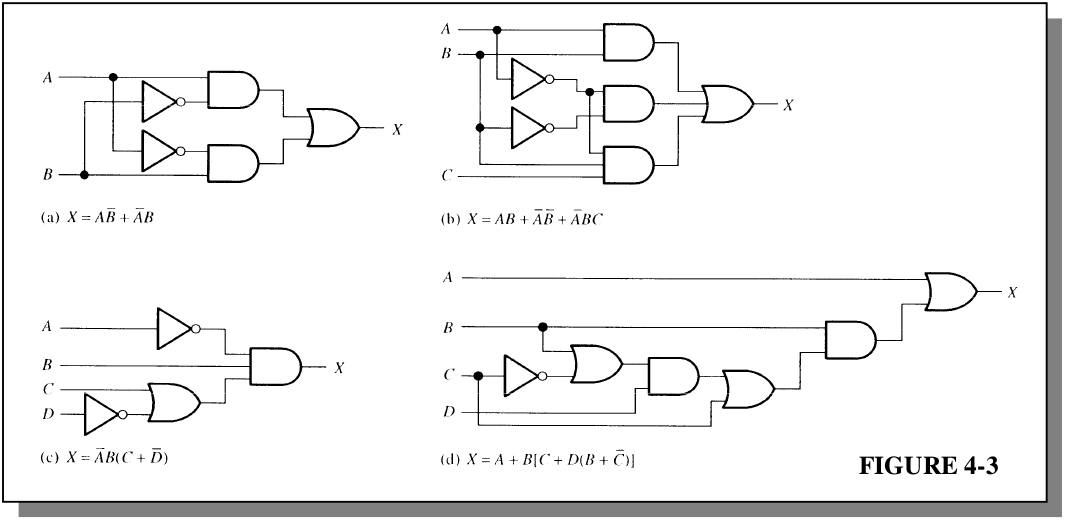
\includegraphics[width=0.45\textwidth]{ex15.png}
\caption{\label{fig:ex15} Answers to Exercise 15.}
\end{figure}
\item Exercise 16: See Fig. \ref{fig:ex16}.
\begin{figure}[ht]
\centering
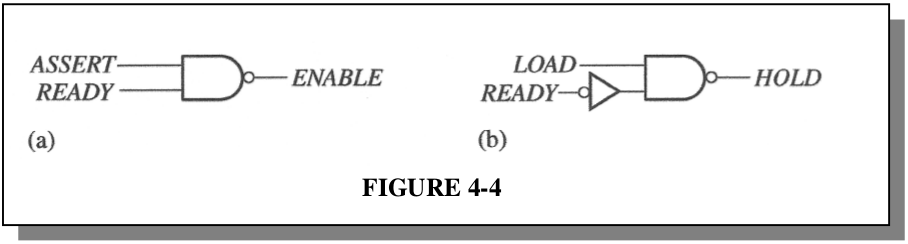
\includegraphics[width=0.55\textwidth]{ex16.png}
\caption{\label{fig:ex16} Answers to Exercise 16.}
\end{figure}
\end{enumerate}

\section{4-5: Logic Simplification Using Boolean Algebra}

\begin{enumerate}
\item Exercise 21: (a) $X = BD + BE + \bar{D}F$ (b) $X = \bar{A}\bar{B}C + \bar{A}\bar{B}D$ (c) $X = B$ (d) $X = AB + CD$ (e) $X = ABC$.
\item Exercise 22: (a) Circuits B and D both reduce to $A\bar{B} + AC\bar{D}$.
\end{enumerate}

\end{document}
